\chapter{Parallel Performance}

\section{Performance}

In computing performance can be defined by two factors,
computational requirements or resources.
Computational requirements can be thought of "what needs to be done?", or efficacy,
and computational resources can be thought in terms of "how much will it cost?", or efficiency.

\begin{equation}
    \mathnormal{Performace} \sim \frac{1}{\mathnormal{Resources~for~solution}}
\end{equation}

\subsection{Expectations}

In a scenario where we have $p$ processors and each processor is rated at $f$ MFLOP, should we see $f \times p$ MFLOPS performance?

The answer is not as simple as "yes".
Several causes may affect performance, while causes may interact with each other,
they need to be understood separately.

\subsection{Embarrassingly Parallel Computations}

Or for short EPCs, are computations that can be trivially divided into several independent parts able to be executed simultaneously.
For \textit{truly} EPCs there should be no interaction between processes, while in \textit{nearly} EPCs the input and output is required to be distributed and combined in some way.

EPCs have potential to achieve maximal speedups in parallel platforms.

\subsection{Scalability}


As previously discussed the performance of a parallel solution is subjected to several factors, namely scalability.
Scalability is the ability of a parallel algorithm of achieving performance gains proportional to the number of processors and the size of the problem.

\paragraph{Evaluation}

To evaluate scalability we can start from the following metrics.

\begin{itemize}
    \item Sequential Runtime ($T_{seq}$) which is a function of problem size and architecture.
    \item Parallel Runtime ($T_{par}$) which is a function of problem size and parallel architecture, that is the number of processors used in execution.
\end{itemize}

With that in mind we can define the speedup $S_p$ as \autoref{eq:speedup},
efficiency $E_p$ as \autoref{eq:efficiency}
and finally the cost $C_p$ as \autoref{eq:cost},
where $p$ is the number of available processors and $T_p$ is the execution time on a $p$ processor system\sidenote{A parallel algorithm is cost-optimal if $C_p = T_1$ or equivalently $E_p = 1$}.

\begin{equation}\label{eq:speedup}
    S_p = \frac{T_1}{T_p}
\end{equation}

\begin{equation}\label{eq:efficiency}
    E_p = \frac{S_p}{p}
\end{equation}

\begin{equation}\label{eq:cost}
    C_p = p \times T_p
\end{equation}

\section{Amdahl's Law}

Amdahl's law fixes the problem size and varies the number of processors,
hence the denomination of Fixed Size Speedup.
The law relates at the reduction of the execution time.
Let $f$ be the sequential fraction of a program, $1-f$ is the part that can be parallelized.

\begin{equation}
    \begin{split}
        S_p & \le \frac{T_1}{T_p} = \frac{T_1}{(f \cdot T_1) + \frac{(1_f)T_1}{p}}\\
        S_p & \le \frac{1}{f + \frac{1-f}{p}}\\
        S_{p \leadsto \infty} & \le \frac{1}{f}
    \end{split}
\end{equation}

\paragraph{Scalability}
When considering scalability, Amdahl's law refers to the abillity of a parallel algorithm to achieve performance gains proportional to the number of processors and the size of the problem.

\paragraph{Application}

Amdahl's law is applicable under the following circumstances:
\begin{itemize}
    \item When the problem size is fixed.
    \item Strong scaling ($p\rightarrow\infty$, $S_p = S_{\infty} \rightarrow \frac{1}{f}$).
    \item Speedup bound is determined by the degree of sequential execution time in the computation.
\end{itemize}

\paragraph{Example}

If $90\%$ of the computation can be parallelized, what is the maximum speedup achievable using 8 processors?

We first calculate the sequential part of the program:

\begin{equation*}
    \begin{split}
        0.9 & = 1 - f\\
        f & = 0.1
    \end{split}
\end{equation*}

And then apply Amdahl's law:

\begin{equation*}
    \begin{split}
        S_8 & \le \frac{1}{0.1 + \frac{1-0.1}{8}}\\
        S_8 & \le 4.7
    \end{split}
\end{equation*}

\section{Gustafson-Barsis’ Law}

\newthought{...speedup should be measured by scaling the
    problem to the number of processors, not by fixing
    the problem size. - John Gustafson}

Also denominated as Scaled Speedup, it is interested in larger problems when scaling.
In other words, for the same time, how much more work can we do?

Considering $a$ the non-parallelizable part and $b$ as the parallelizable part,
we calculate $T_P$, for $P$ processors, as follows:
\begin{equation}
    \begin{split}
        T_P & = a + P \cdot b\\
        T_1 & = a + 1 \cdot b\\
            & = a + b
    \end{split}
\end{equation}

Given that the wall-clock execution time is always the same,
the scaled speedup is calculated on the volume of data processed.

\begin{equation}
    \begin{split}
        S_P & \le \frac{T_P}{T_1}\\
        & \le \frac{a + P \cdot b}{a + b}
    \end{split}
\end{equation}

Consider $\alpha = \frac{a}{a+b}$ as the sequential fraction of the parallel execution time.
We can then define the scaled speedup as follows:

\begin{equation}
    \begin{split}
        S_P & \le \alpha + P \cdot (1-\alpha)\\
        & \le P - \alpha \cdot (P-1)
    \end{split}
\end{equation}

\paragraph{Scalability}
The ability of a parallel algorithm to achieve performance gains proportional to the number of processors and the size of the problem.

\paragraph{Application}

The Gustafson’s law applies under the following scenarios:
\begin{itemize}
    \item When the problem size can increase.
    \item When the number of processors increases.
    \item Speedup function include the number of processors.
    \item Can maintain or increase parallel efficiency as the problem scales.
\end{itemize}

\paragraph{Example} An application executing on $64$ processors spends $5\%$ of the total time on non-parallelizable computations.
What is the scaled speedup?

\begin{equation}
    \begin{split}
        S_64 & \le P - \alpha \cdot (P-1)\\
             & \le 64 - 0.05 \cdot (64 - 1)\\
             & \le 60.85
    \end{split}
\end{equation}

\section{Computational DAG}

A parallel program maybe be represented as a directed acyclic graph (DAG),
this graph has several properties, such as the span,
which can be used to evaluate the potential performance of an algorithm.

\begin{figure}
    \centering
    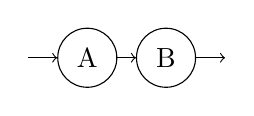
\begin{tikzpicture}
        \node[name=a, draw, circle, minimum size=0.75cm] at (0,0) {A};
        \node[name=b, draw, circle, minimum size=0.75cm] at (1,0) {B};
        \draw[->] (-.75, 0) -- (a);
        \draw[->] (a) -- (b);
        \draw[->] (b) -- (1.75,0);
    \end{tikzpicture}
    \caption{Serial Composition}
    \label{fig:dag:serial}
\end{figure}


\begin{figure}
    \centering
    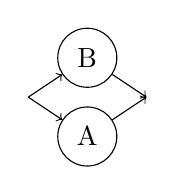
\begin{tikzpicture}
        \node[name=a, draw, circle, minimum size=0.75cm] at (0,0) {A};
        \node[name=b, draw, circle, minimum size=0.75cm] at (0,1) {B};
        \draw[->] (-.75, 0.5) -- (a);
        \draw[->] (-.75, 0.5) -- (b);
        \draw[->] (a) -- (.75, 0.5);
        \draw[->] (b) -- (.75, 0.5);
    \end{tikzpicture}
    \caption{Parallel Composition}
    \label{fig:dag:parallel}
\end{figure}

\paragraph{Work}

The total number of tasks of the graph is called \textit{work},
this is equivalent to running the algorithm with a single processing unit ($T_1$).

\begin{equation}\label{eq:work_law}
    T_p \ge \frac{T_1}{P}
\end{equation}

The work is equal whether considering $T_1$ or $T_P$,
that is:

\begin{equation}
    T_1 (A \cup B) = T_1(A) + T_1(B)
\end{equation}

\paragraph{Span}

The span, or the critical-path length, is the minimum of sequential steps the algorithm must execute.

\begin{equation}\label{eq:span_law}
    T_p \ge T_{\infty}
\end{equation}

The span is different when comparing $T_1$ and $T_P$.

\begin{equation}
    \begin{split}
        T_{\infty} (A \cup B) & = T_{\infty}(A) + T_{\infty}(B)\\
        T_{\infty} (A \cup B) & = max\{T_{\infty}(A), T_{\infty}(B)\}\\
    \end{split}
\end{equation}

\subsection{Speedup}

The speedup on $P$ processors is given by:

\begin{equation}
    \frac{T_1}{T_P}
\end{equation}

If $\frac{T_1}{T_P} = P$ we have \textit{linear} speedup.
When $\frac{T_1}{T_P} \ge P$ we have \textit{superlinear} speedup,
this however is not possible due to the work law (\autoref{eq:work_law}).

\subsection{Parallelism}

Parallelism can be defined as the average amount of work per step along the span, that is:

\begin{equation}
    \frac{T_1}{T_\infty}
\end{equation}

\subsection{Work-Span Model}

Considers a greedy scheduler, that is,
no worker is idle while there are tasks to execute.

\begin{itemize}
    \item $T_P$ - running time with $P$ workers.
    \item $T_1$ - running time with 1 worker, serial execution.
    \item $T_\infty$ - the time taken along the critical path.
\end{itemize}

The critical path is the sequence of tasks that has the longest execution time.

\paragraph{Lower-Bound}
A lower-bound can be calculated with the following formula:

\begin{equation}
    \mathnormal{max}\left(\frac{T_1}{P}, T_\infty\right) \le T_P
\end{equation}

\paragraph{Upper-Bound}

\begin{equation}
    T_P \le \frac{T_1 - T_\infty}{P + T_\infty}
\end{equation}